

\section{Overview}
The agriculture industry is highly reliant on water for crop production and food supply. Around 70\% of fresh water used globally is used for agriculture \citep{emily_2023}, and farms depend on reliable water supply to irrigate crops regularly and ensure that their supply meets the industry's demand. Severe rainfall variability damages not only a farmer's yield and agricultural output, but also a household's dietary diversity \citep{object_object_2020}, which is necessary for proper "nutrition and overall well-being" \citep{food_diversity}.

Rainfall variability has been shown to "frequently undermine farm yields, reduce food availability, and lower income" \citep{guido_zimmer_lopus_hannah_gower_waldman_krell_sheffield_caylor_evans_2020}. This is not limited to periods of low rainfall, but also periods of high rainfall, which can "increase agricultural runoff", "harm water quality", and hamper crop production by damaging the soil on which they are grown. These problems are only exacerbated as climate change becomes an increasingly pressing issue \citep{united_states_environmental_protection_agency_2025} and rainfall variability is increased. For farmers in area of high water volatility, the need for reliable information on water levels is growing. 

By enabling farmers to capture and store water during periods of high availability (such as winter rainfall or peak streamflow), these reservoirs provide a vital supply for irrigation and other needs during drier periods, effectively smoothing seasonal supply-demand imbalances caused by rainfall variability. This reduces reliance on potentially costly mains water or direct abstraction during sensitive summer months, offering greater protection against drought and supporting consistent crop production.

In the UK, small farm water reservoirs under 25,000 cubic metres \citep{ukgov_2014_reservoirs} do not require permits. This could raise potential risks to the environment, as with more non-permit, non-registered water reservoirs, there are more likely to be adverse effects on the local water cycle due to unpredictable levels of water abstraction being carried out. For this reason, it would be beneficial for governments to have the ability to map these small farm water reservoirs. One method of doing this is through analysis of satellite data with a classification model able to identify and note the size and location of water reservoirs, particularly in east England. 

Recognising the importance of this on-farm infrastructure for both food security and environmental management, UK government policy initiatives actively encourage the development of water storage solutions. Schemes like the Water Management Grant, part of the Farming Investment Fund, offer financial support to farmers for constructing reservoirs and investing in efficient irrigation systems \citep{ruralpaymentsagency_2023}, aiming to promote sustainable water use. These initiatives align with broader governmental goals, such as Defra's aim to significantly increase the amount of water stored by the farming sector by 2050 \citep{andcornwall_2024}. Additionally, collaborative approaches like multi-farm reservoirs and water sharing schemes \citep{for_2024} are being explored through dedicated funding to further enhance regional water management resilience.

\section{Problem Addressed}
While many large water reservoirs and water abstraction operations are licensed and monitored, a significant data gap exists regarding the prevalence and distribution of small, unregistered reservoirs on UK farms. This lack of knowledge is problematic for several key reasons. Firstly, without a comprehensive register of these smaller reservoirs, it becomes impossible to accurately assess the true uptake of on-farm water storage solutions or evaluate the effectiveness of policy initiatives designed to encourage their sustainable growth. Secondly, although individual small reservoirs fall below regulatory thresholds and may primarily fill during wetter periods, their cumulative impact is unknown. Unmonitored proliferation could potentially lead to significant alterations in local hydrological cycles and unforeseen environmental sustainability issues, even if individual abstractions seem minor. Finally, this data gap hinders effective water resource management and regulatory oversight. If the locations and number of these reservoirs are unknown, authorities cannot verify whether abstraction rules, such as permitted filling times, are being adhered to, potentially undermining efforts to manage water resources sustainably, especially given that some abstraction practices are already known to be unsustainable \citep{departmentofenvironmentfoodandruralaffairs_2019_abstraction}.

To ensure responsible retention, usage, or disposal of immediate-use abstracted and reservoir-stored water, it is first necessary to have an accurate register of the reservoirs in the country. Travelling to each farm and identifying whether or not they use a water reservoir is a costly and time-consuming endeavour. Additionally, these types of visits would have to be regular enough so that the filling and release of water can be monitored as well. For a resource and staff-constrained agency such as the Environmental Agency (EA), \citep{comptrollerandauditorgeneral_2022}, it is impossible to have enough enforcers to go out checking every farm. This problem is further exacerbated by the steadily declining funding the the EA has been receiving in recent years demonstrated in figure \ref{fig:EA funding decline}. 

\begin{figure}[ht]
    \centering
    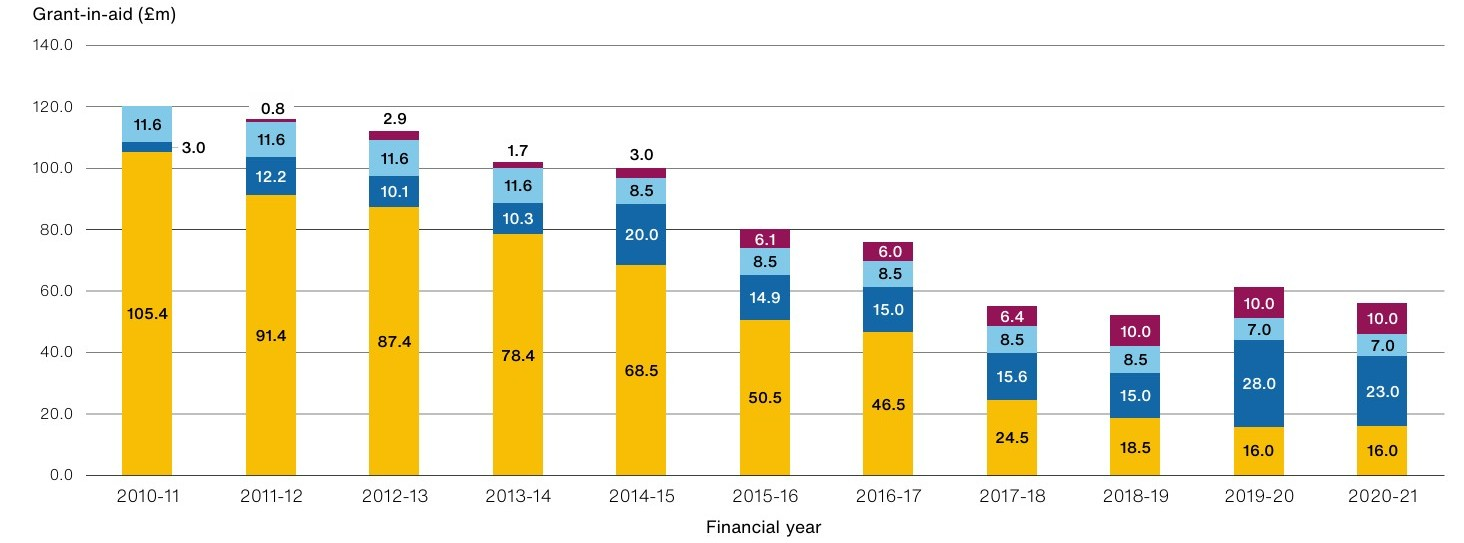
\includegraphics[width=0.5\linewidth]{contents/figures/intro-environment agency funding.jpg}
    \caption{"Grant-in-aid funding to the Environment Agency for environmental protection, 2010-11 to 2020-21" \citep{comptrollerandauditorgeneral_2022}}
    \label{fig:EA funding decline}
\end{figure}

Given the challenges and potential inaccuracies associated with ground-based monitoring for numerous small, unregistered reservoirs, alternative approaches are needed. Satellite remote sensing, the science of acquiring information about the Earth's surface by "measuring reflected and emitted radiation at a distance" \citep{usgs_2022a}, offers significant potential as a monitoring tool, providing wide-area coverage repeatably and often more cost-effectively than extensive field surveys, especially for monitoring change over time. However, raw satellite imagery requires sophisticated analysis to extract meaningful information.

Therefore, it would be beneficial to develop specialised algorithms capable of processing these datasets to automatically identify potential water reservoirs on farms. Critically, such algorithms must go beyond simple water detection; the model should also be able to differentiate water body features that resemble, and are most likely to be, constructed farm reservoirs from other water bodies (like rivers, ponds, or flooded areas) and non-water features that might appear spectrally similar. Furthermore, for these advanced remote sensing methods to be truly impactful, the development of robust algorithms must be accompanied by accessible tools and clear methodologies. This is essential to translate complex satellite data and model outputs into practical, actionable information that can be readily used by policymakers, regulatory bodies like the Environment Agency, and water resource managers to monitor reservoir distribution, assess compliance, and evaluate the effectiveness of water management policies.

The main beneficiary for this project is likely to be a government body seeking to identify unpermitted reservoirs that pose potential risks to the water cycle or nearby ecosystems. 

\section{Aim and Objectives}
The aim for this project is to investigate the quantity, location, and size of small farm water reservoirs in the east of England. To do this, I will develop and train a machine learning classification model that uses satellite imagery data to identify water reservoirs. The model should also be able to differentiate water reservoirs from other non-reservoir water bodies. The remaining third class will be composed of land types that contain neither. 

I have defined four objectives that shall be achieved to ensure successful development and training of the classification model: 
\begin{enumerate}
    \item Select one appropriate satellite image for the development of the necessary software tools and three more satellite images for model deployment. 

    The singular development image is intended for building the programs around a generic satellite image (specifically Sentinel 2), while the three deployment images are for validating the program under different conditions. 
    \item Develop a software tool to automate satellite imagery handling/pre-processing and facilitate the semi-automated creation of labelled training data through a dedicated user interface. 
    
    Satellite imagery handling includes automatic file search given a directory, cloud masking, index calculation, data file preparation, and response data saving. 
    \item Build, train, and validate a machine learning classification model (specifically using the Keras Sequential model) for water reservoirs, non-reservoir water bodies, and land.
    \item Deploy the model over East England and produce a map of the quantity, location, and size of all water reservoirs in East England for March 2025. 
\end{enumerate}

The following section will explain and justify the study area and time period selected for these objectives.

\section{Study Area and Time Period}
As can be seen from the final objective, the study area is East England, and the time period was selected as the month of March in 2025. 

This study area was selected because East England, together with the East Midlands, contributes the highest total income from farming in the UK \citep{defra_2024}, indicating the greatest density of agricultural holdings and thus the most small reservoirs to detect. Moreover, East Anglia is among the driest regions of the country \citep{matthew_de-machen_mjr.global_2024} and already under acute pressure from summer water shortages; it accounts for the highest irrigation abstractions in England and Lincolnshire, and its farms are most exposed to drought risk \citep{ukia_2024, johns_2023}. 

Climate projections and recent observations signal widening supply–demand gaps: by 2050, summer water deficits in England could approach five billion litres per day during dry spells, potentially triggering hosepipe bans and prioritisation conflicts between public supply and agriculture \citep{horton_2024}. Concurrently, modelling under a range of socio-economic and climate scenarios, forecasts estimate that irrigation demand in East Anglia may rise 10 to 40 percent by 2050, driven by hotter, drier summers and evolving cropping patterns \citep{henriques_holman_audsley_pearn_2008, uk_ceh_2025}. 

These intersecting factors, high farm density, the driest UK climate, and escalating water use demands, make East England the ideal test-bed for an automated reservoir-mapping tool that supports regional water‐management and drought‐resilience planning.

This time period was finalised and selected to simplify data handling was much as possible. March 2025 was "the sunniest March" since records began \citep{pressoffice_2025_a}, making it ideal for satellite imagery. Clouds in satellite imagery are problematic because they can largely obscure important information on the ground. There are some strategies to mitigate these problems, which will be covered in the Methodology section, however the simplest way to avoid the problem altogether is to select images with the lowest cloud cover percentage. Selecting March as the month of choice is optimal as it guarantees a larger proportion of the images selected will be only minimally covered by clouds. 

\subsection{To what extent is this problem global?}
While this study focuses on East England as a case study/proof-of-concept, the problem of needing to efficiently identify and monitor small water reservoirs is a widespread global challenge relevant to agriculture, environment, and water management. This study demonstrates a scalable technical solution using globally available data and techniques, proving that this machine learning approach can be effectively implemented to tackle this global problem.

\section{Dissertation Structure}
I will now provide a brief overview of the contents of each section in this report. 
\subsection{Literature Review}
\subsection{Methodology}
\subsection{Results}
\subsection{Discussion}
\subsection{Conclusion}